\documentclass[10pt,twoside]{article}

\usepackage[T1]{fontenc}
\usepackage[scaled]{uarial}
\renewcommand{\familydefault}{\sfdefault}
\usepackage{tgadventor}
\usepackage{amsfonts}
\usepackage{amssymb}
\usepackage{amsmath}
\usepackage{listings}
\usepackage{array}
\usepackage[margin=2.54cm]{geometry}
\usepackage{fancyhdr}
\usepackage{graphicx}
\usepackage{titlesec}
\usepackage{setspace}
\usepackage{parskip}
\usepackage{lmodern}


\begin{document}

\begin{titlepage}
    \centering
    
\includegraphics{logo.png}\par\vspace{1cm}
    {\scshape\Large Università degli Studi di Padova \par}
    \vspace{1.5cm}
    {\scshape\large Dipartimento di Matematica\par}
    \vspace{0.5cm}
    {\scshape\large Laurea Triennale in Informatica\par}
    \vspace{2cm}
    {\scshape\Large Progetto di Basi di Dati\\\par}
    \vspace{1cm}
    \hrule
    \vspace{1cm}
    {\large\bfseries
    Basi di Dati di un Sistema Informativo\\
    per la Gestione di una Scuola Guida\par}
    \vspace{1cm}
    \hrule
    \vfill
    {\large Andrea Difino, Davide Colabove\par}
\end{titlepage}

\pagestyle{fancy}
\fancyhead{}
\fancyhead[C]{\fontsize{9}{9}\selectfont Progetto di una Base di Dati di un Sistema Informativo per la Gestione Scuola Guida}
\title{\fontsize{12}{12}\selectfont A.A. 2024/25 \\ Corso di Laurea in Scienze e Tecnologie Informatiche SC1167}
\date{}
\maketitle

\renewcommand{\contentsname}{Indice}
\tableofcontents

\newpage

\section{Abstract}{
    Questo lavoro sviluppa una base di dati progettata per gestire in modo strutturato e coerente le informazioni relative alle scuole guida, agli istruttori, agli iscritti ai corsi e agli esami sostenuti dagli allievi. 
    
    L’obiettivo principale è fornire un sistema che supporti le attività di pianificazione, monitoraggio e ottimizzazione delle risorse didattiche, garantendo un accesso organizzato ai dati e facilitando la loro analisi.

    Nel contesto della formazione alla guida, la base di dati proposta distingue tra lezioni teoriche e pratiche, gestendo attributi specifici quali assegnazione di aule, veicoli disponibili e disponibilità degli istruttori. Gli iscritti sono tracciati in base ai percorsi di formazione intrapresi e ai risultati degli esami, con particolare attenzione alle performance nelle prove teoriche e pratiche. Il sistema registra anche le prenotazioni delle lezioni e i pagamenti associati ai servizi offerti.

    Questa base di dati è progettata per garantire un’archiviazione efficiente e strutturata delle informazioni formative, migliorando il recupero e l’analisi dei dati. L’organizzazione sistematica delle informazioni contribuisce a un utilizzo più efficace delle risorse didattiche, ottimizzando la gestione delle scuole guida e supportando i processi decisionali.

}

\section{Analisi dei Requisiti}{
    Questa sezione riassume i requisiti a cui deve sottostare la base di dati.

    \paragraph{Iscritto.}
    Gli iscritti sono le persone che frequentano i corsi della scuola guida e sono identificati attraverso:

    \begin{itemize}
        \item Codice Fiscale (identificativo univoco).
        \item Nome.
        \item Cognome.
        \item Numero di telefono.
        \item Indirizzo email.
        \item Città e indirizzo di residenza.
        \item Categoria di patente richiesta (A, B, C, ecc.).
        \item Data di iscrizione.
    \end{itemize}
    
    Ogni iscritto può partecipare a più lezioni teoriche e pratiche, sostenere più esami, e può lasciare recensioni su lezioni o istruttori.
    

    \paragraph{Istruttore.}
    Gli istruttori sono i docenti responsabili delle lezioni e sono descritti tramite:
    
    \begin{itemize}
        \item Codice Fiscale (identificativo univoco).
        \item Nome.
        \item Cognome.
        \item Numero di telefono.
        \item Indirizzo email.
        \item Anni di esperienza professionale.
        \item Categorie di patente per cui sono abilitati all’insegnamento.
    \end{itemize}

    Un istruttore può tenere più lezioni sia teoriche che pratiche, ma non può essere assegnato contemporaneamente a due lezioni sovrapposte.
    

    \paragraph{Veicolo.}
    I veicoli sono utilizzati per le lezioni pratiche e per gli esami pratici. Per ogni veicolo vengono registrate le seguenti informazioni:
    
    \begin{itemize}
        \item Targa (identificativo univoco).
        \item Modello.
        \item Tipo di veicolo (Auto, Moto, ecc.).
        \item Anno di immatricolazione.
        \item Stato operativo (disponibile, in manutenzione, non disponibile).
    \end{itemize}

    Ogni veicolo può essere utilizzato in più lezioni pratiche o esami pratici. Tuttavia, ogni lezione pratica o esame pratico è associato a un solo veicolo alla volta.
    

    \paragraph{Aula.}
    Le aule sono gli spazi in cui si svolgono le lezioni teoriche e sono caratterizzate da:

    \begin{itemize}
        \item Nome aula. (identificativo univoco)
        \item Numero di posti disponibili.
        \item Tipologia di attrezzatura didattica disponibile (proiettore, lavagna, ecc.).
    \end{itemize}

    Un’aula può ospitare più lezioni, ma non contemporaneamente.
    

    \paragraph{Lezione.}
    Le lezioni rappresentano le attività formative offerte dalla scuola guida e sono caratterizzate da: 
    
    \begin{itemize}
        \item Ora inizio lezione.
        \item Data.
        \item Argomento lezione.
    \end{itemize}
    
    si suddivide in:

    \begin{itemize}
        \item Lezione teorica:
        \item Lezione pratica che aggiunge:
        \begin{itemize}
            \item Durata.
        \end{itemize}
    \end{itemize}

    Ogni lezione ha un solo istruttore assegnato. Le lezioni teoriche possono avere più iscritti, mentre quelle pratiche sono individuali.
    

    \paragraph{Prenotazione.}
    Le prenotazioni associano un iscritto a una lezione:

    \begin{itemize}
        \item Data di prenotazione. 
        \item Stato della prenotazione (confermata, annullata, in attesa).
    \end{itemize}

    Un iscritto può prenotare più lezioni.
    

    \paragraph{Esame.}
    Gli esami valutano la preparazione degli iscritti e sono caratterizzati da:

    \begin{itemize}
            \item Data dell’esame.
            \item Esito (superato o non superato).
            \item Durata
    \end{itemize}

    si suddivide in: 

    \begin{itemize}
        \item Esame teorico:
        \begin{itemize}
            \item Sede
            \item Punti
        \end{itemize}
        \item Esame pratico
    \end{itemize}

    Un iscritto può sostenere più tentativi di esame. 


    \paragraph{Recensione.}
    Gli iscritti possono lasciare recensioni relative a:

    \begin{itemize}
        \item Una lezione frequentata.
        \item Un istruttore con cui hanno svolto lezioni.
    \end{itemize}

    Per ogni recensione sono registrati:

    \begin{itemize}
        \item Data della recensione.
        \item Gradimento (da 1 a 5 stelle).
        \item Commento testuale.
        \item Oggetto 
    \end{itemize}

    Un iscritto può recensire un istruttore o una lezione.


    \paragraph{Pagamento.}
    Gli iscritti devono effettuare i pagamenti relativi ai servizi formativi:

    \begin{itemize}
        \item Data di pagamento.
        \item Importo versato.
        \item Metodo di pagamento (carta di credito, bonifico, contante).
        \item Stato del pagamento (pagato, da pagare).
    \end{itemize}

    Ogni pagamento è associato a un singolo iscritto.

}

\newpage

\section{Progettazione Concettuale}{
    \subsection{Lista Entità}{
        Esistono esattamente due tipi di lezioni, teoriche e pratiche.

        Ogni lezione pratica prevede l'assegnazione di un veicolo specifico e la partecipazione di un singolo iscritto per volta, mentre le lezioni teoriche si svolgono in un'aula e possono coinvolgere più iscritti contemporaneamente.

        Gli istruttori sono responsabili della conduzione delle lezioni: ogni istruttore può tenere sia lezioni teoriche che pratiche, ma non può essere assegnato a più lezioni contemporaneamente.
        Gli iscritti sono gli allievi della scuola guida e possono prenotare lezioni, sostenere esami, e lasciare recensioni sugli istruttori o sulle lezioni frequentate.

        L’analisi dei requisiti dà particolare enfasi agli esami pratici, i quali prevedono l’uso obbligatorio di un veicolo assegnato; per questo motivo, il concetto di esame pratico viene rappresentato come un'estensione dell'esame, caso particolare dell'esame generale.
        In particolare, si tiene traccia degli esami pratici svolti con uno specifico veicolo, registrando l’esito della prova.

        Ogni prenotazione associa un iscritto a una lezione, garantendo la corretta gestione delle disponibilità di istruttori, aule e veicoli.
        Analogamente, ogni pagamento è riferito a un iscritto e rappresenta una transazione economica per il servizio formativo ricevuto.

        Tabella 1 (descritta successivamente) riassume tutte le entità e relazioni individuate dall'analisi dei requisiti e rappresentate nel diagramma E-R, con i relativi attributi rilevanti.
        Per le entità principali viene anche fornito l'identificatore, che può includere riferimenti a relazioni nei casi di Lezione, Esame, Prenotazione e Pagamento.

        Il presente schema E-R non permette di rappresentare direttamente il seguente vincolo di business:

        $$
        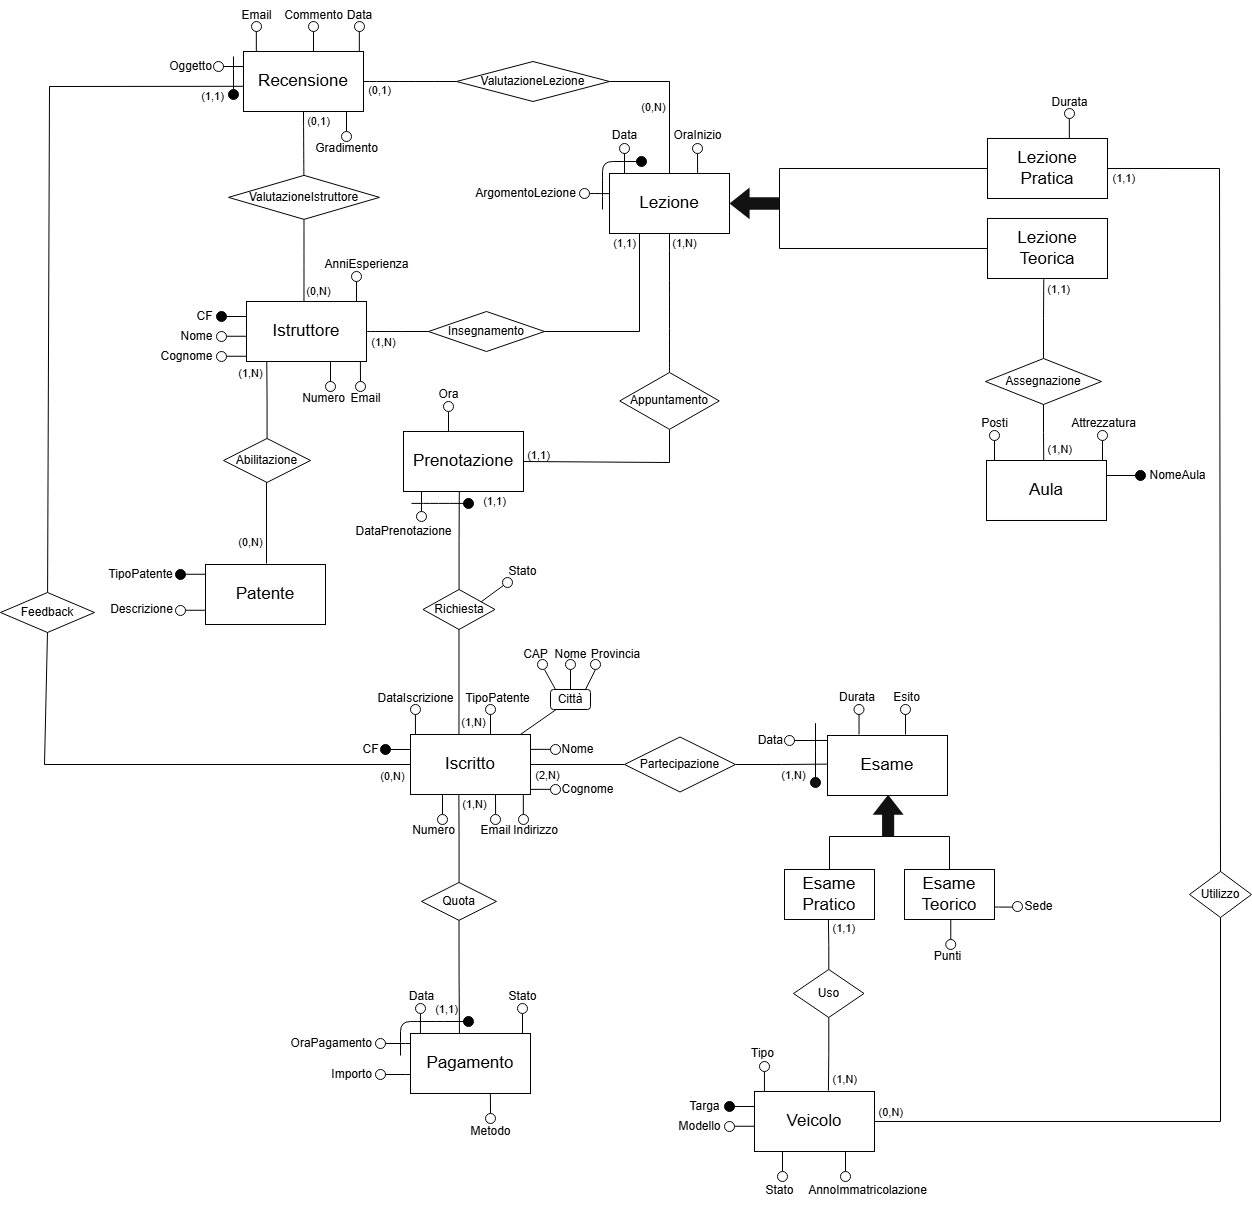
\includegraphics[width=.70\linewidth]{img/ER_ScuolaGuida.drawio.png}
        $$
    }
}
\end{document}